% 
%            ,,                                        
%          `7MM            _.o9                                
%            MM                                             
%  ,6"Yb.    MM  ,p6"bo   ,6"Yb.  M"""MMV  ,6"Yb.  `7Mb,od8 
% 8)   MM    MM 6M'  OO  8)   MM  '  AMV  8)   MM    MM' "' 
%  ,pm9MM    MM 8M        ,pm9MM    AMV    ,pm9MM    MM     
% 8M   MM    MM YM.    , 8M   MM   AMV  , 8M   MM    MM     
% `Moo9^Yo..JMML.YMbmd'  `Moo9^Yo.AMMmmmM `Moo9^Yo..JMML.   
% 
% 
% Free, Open-Source Thesis template for LaTeX
% https://github.com/dpmj/alcazar


% %%%%%%%%%%%%%%%%%%%%%%%%%%%%%%%%%%%%%%%%%%%%%%%%%%%%%%%%%%%%%%%%%%%%%%%%%%%%%%
% PREAMBLE

\documentclass[twoside, openright, 12pt, final]{report}


% ------------------------------------------------------------------------------
% Variables

% Title for the title page 
\newcommand{\thesisTitle}{Alcázar: a free and open source template for academic papers, for nerdy kids who do boring stuff like theses with endless titles.}
% Title for the pages' heading 
\newcommand{\thesisTitleShort}{Alcázar: a free and open source template for academic works.}

\newcommand{\thesisType}{Master's Thesis}  % Bachelor's Thesis, Master's Thesis, PhD Thesis...
\newcommand{\thesisDegree}{Master's Degree}  % Bachelor's Degree, Master's Degree, PhD...
\newcommand{\thesisArea}{Typesetting Engineering}  % Area of knowledge

\newcommand{\thesisAuthor}{Name of the author of the thesis}
\newcommand{\thesisTutor}{Name of the supervisor of the thesis}  

\newcommand{\thesisYear}{2077}  % Date of the thesis' submission or defense 
\newcommand{\thesisMonth}{June}
\newcommand{\thesisDate}{{\thesisMonth} {\thesisYear}}
\newcommand{\thesisAcademicCourse}{2076/2077}  % During which academic year(s) was the thesis developed

\newcommand{\thesisSchool}{University of Misco}
\newcommand{\thesisAddress}{Fake avenue 00, Region, Country}
\newcommand{\thesisDepartment}{Based department}

\newcommand{\thesisKeywords}{Keyword 1, Keyword 2, Keyword 3, Keyword 4, Keyword 4, Keyword 5, Keyword 6, Keyword 7, Keyword 8, Keyword 9, Keyword 10, Keyword N}  
% For the abstract and indexing

% ------------------------------------------------------------------------------
% Import document style
\usepackage{style/alcazar}


% END PREAMBLE
% %%%%%%%%%%%%%%%%%%%%%%%%%%%%%%%%%%%%%%%%%%%%%%%%%%%%%%%%%%%%%%%%%%%%%%%%%%%%%%
% BEGIN DOCUMENT

\begin{document}

% Titlepage, license, about, abstract, keywords, publications, acknowledgements, dedication and tables of contents
% 
%            ,,                                        
%          `7MM            _.o9                                
%            MM                                             
%  ,6"Yb.    MM  ,p6"bo   ,6"Yb.  M"""MMV  ,6"Yb.  `7Mb,od8 
% 8)   MM    MM 6M'  OO  8)   MM  '  AMV  8)   MM    MM' "' 
%  ,pm9MM    MM 8M        ,pm9MM    AMV    ,pm9MM    MM     
% 8M   MM    MM YM.    , 8M   MM   AMV  , 8M   MM    MM     
% `Moo9^Yo..JMML.YMbmd'  `Moo9^Yo.AMMmmmM `Moo9^Yo..JMML.   
% 
% 
% Free and Open-Source template for academic works
% https://github.com/dpmj/alcazar



% Title page
% 
%            ,,                                        
%          `7MM            _.o9                                
%            MM                                             
%  ,6"Yb.    MM  ,p6"bo   ,6"Yb.  M"""MMV  ,6"Yb.  `7Mb,od8 
% 8)   MM    MM 6M'  OO  8)   MM  '  AMV  8)   MM    MM' "' 
%  ,pm9MM    MM 8M        ,pm9MM    AMV    ,pm9MM    MM     
% 8M   MM    MM YM.    , 8M   MM   AMV  , 8M   MM    MM     
% `Moo9^Yo..JMML.YMbmd'  `Moo9^Yo.AMMmmmM `Moo9^Yo..JMML.   
% 
% 
% Free and Open-Source template for academic works
% https://github.com/dpmj/alcazar


% ------------------------------------------------------------------------------
% Title page

\thispagestyle{empty}

\pagenumbering{roman}
\setcounter{page}{1}

\newgeometry{
    left    = 3.0cm,
    right   = 3.0cm,
    top     = 3.5cm,
    bottom  = 3.5cm
}

\begin{center}
    \includegraphics[height=13mm]{opening/resources/logos/logo_upv.pdf}  % 13 mm, 15 mm, etc.
    \hfill
    \includegraphics[height=13mm]{opening/resources/logos/logo_upv_telcom.pdf}
\end{center}

\vspace*{30mm}

\begin{center}
    \textbf{\large \textsc{{\thesisDegree} in}}\\
    \textbf{\large \textsc{\thesisArea}}
\end{center}

\vspace*{0mm}

\begin{center}
    \textbf{\large \thesisType}
\end{center}

\vspace*{10mm}

\begin{center}
    \setstretch{1.7}
    \textbf{{\LARGE {}``\thesisTitle''}}\\
\end{center}

\vspace*{15mm}

\begin{center}
    {\large \textsc{Academic course:} \thesisAcademicCourse}
\end{center}

\vspace*{15mm}

\begin{center}
    AUTHOR:
    \par
    \textbf{{\large \thesisAuthor}}
\end{center}

\begin{center}
    TUTOR:
    \par
    \textbf{{\large \thesisTutor}}
\end{center}

\begin{center}
    \vspace*{1mm}
    {\large \thesisDepartment}
\end{center}

\newpage
\thispagestyle{empty}
\restoregeometry


% License
% 
%            ,,                                        
%          `7MM            _.o9                                
%            MM                                             
%  ,6"Yb.    MM  ,p6"bo   ,6"Yb.  M"""MMV  ,6"Yb.  `7Mb,od8 
% 8)   MM    MM 6M'  OO  8)   MM  '  AMV  8)   MM    MM' "' 
%  ,pm9MM    MM 8M        ,pm9MM    AMV    ,pm9MM    MM     
% 8M   MM    MM YM.    , 8M   MM   AMV  , 8M   MM    MM     
% `Moo9^Yo..JMML.YMbmd'  `Moo9^Yo.AMMmmmM `Moo9^Yo..JMML.   
% 
% 
% Free and Open-Source template for academic works
% https://github.com/dpmj/alcazar


%%%%%%%%%%%%%%%%%%%%%%%%%%%%%%%%%%%%%%%%%%%%%%%%%%%%%%%%%%%%%%%%%%%%%%%%%%%%%%%%%%%%%%%%%%%%
% LICENSE

\newpage
\thispagestyle{empty}

\vspace*{\fill}

\begingroup

    \setlength\tabcolsep{0pt}
    \renewcommand*{\arraystretch}{1.4}
    \renewcommand{\baselinestretch}{0.9}\footnotesize  % Comprime space
    
    \noindent
    \begin{tabular}{m{3.5cm} m{11.5cm}}
        \includegraphics[width=3cm]{opening/resources/license/by-sa.pdf} & {\normalsize {\thesisAuthor} and {\thesisTutor}} \\
    \end{tabular}
    
    \noindent This work is licensed under the Creative Commons Attribution-ShareAlike 4.0 International (CC BY-SA 4.0) license. This is a human-readable summary of (and not a substitute for) the license. You are free to:
    
    \noindent
    \begin{tabular}{m{1.5cm} m{13.5cm}}
        \textbf{Share} & Copy and redistribute the material in any medium or format.\\
        \textbf{Adapt} & Remix, transform, and build upon the material.\\
    \end{tabular}
    
    \vspace{1mm}
    
    \noindent The licensor cannot revoke these freedoms as long as you follow the license terms:
    
    \noindent
    \begin{tabular}{m{1.5cm} m{13.5cm}}
        
\includegraphics[width=2em]{opening/resources/license/by.pdf} & \textbf{Attribution:} You must give appropriate credit, provide a link to the license, and indicate if changes were made. You may do so in any reasonable manner, but not in any way that suggests the licensor endorses you or your use.\\
        
\includegraphics[width=2em]{opening/resources/license/sa.pdf} & \textbf{ShareAlike:} If you remix, transform, or build upon the material, you must distribute your contributions under the same license as the original.
    \end{tabular}
    
    \noindent To view a complete copy of this license, visit 
    \href{https://creativecommons.org/licenses/by-nc-sa/4.0/}{https://creativecommons.org/licenses/by-sa/4.0}

\endgroup


% Give a little credit to the template :)
% It's completely optional, of course ;)

\begingroup

    \vspace*{2mm}

    \setlength\tabcolsep{0pt}
    \renewcommand*{\arraystretch}{1.4}
    \renewcommand{\baselinestretch}{0.9}\footnotesize  % Comprime space
    
    \noindent
    \begin{tabular}{m{3.5cm} m{11.5cm}}
        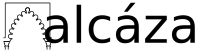
\includegraphics[width=3cm]{opening/resources/logos/alcazar.pdf} & \noindent This document has been generated using {\href{https://github.com/dpmj/alcazar}{Alcázar}}, a free and open source {\LaTeX} template for academic works by \href{https://www.linkedin.com/in/dpmj/}{Juan Del Pino Mena}. \\
    \end{tabular}

    

\endgroup




% About the document
% Collaborators, repositories, social networks, links, etc.
% Feel free to edit this doc:
% 
%            ,,                                        
%          `7MM            _.o9                                
%            MM                                             
%  ,6"Yb.    MM  ,p6"bo   ,6"Yb.  M"""MMV  ,6"Yb.  `7Mb,od8 
% 8)   MM    MM 6M'  OO  8)   MM  '  AMV  8)   MM    MM' "' 
%  ,pm9MM    MM 8M        ,pm9MM    AMV    ,pm9MM    MM     
% 8M   MM    MM YM.    , 8M   MM   AMV  , 8M   MM    MM     
% `Moo9^Yo..JMML.YMbmd'  `Moo9^Yo.AMMmmmM `Moo9^Yo..JMML.   
% 
% 
% Free and Open-Source template for academic works
% https://github.com/dpmj/alcazar

\newpage
\pagestyle{empty}

\clearpage
\cleardoublepage
\phantomsection

\pagestyle{empty}

\phantomsection
\addcontentsline{toc}{chapter}{About the authors}


%%%%%%%%%%%%%%%%%%%%%%%%%%%%%%%%%%%%%%%%%%%%%%%%%%%%%%%%%%%%%%%%%%%%%%%%%%%%%%%%%%%%%%%%%%%%
% ABOUT THE AUTHORS


% \vspace*{\fill}

\begingroup

    \footnotesize
    \setlength\tabcolsep{0pt}
    \renewcommand*{\arraystretch}{1}
    
    \noindent
    \begin{tabular}{p{3cm} p{12cm}}
        \vspace{0mm} \includegraphics[width=2.5cm]{opening/resources/about/coomer.png}
        \newline
        & \vspace{-0.5mm} {\normalsize \bf \thesisAuthor}
        \hfill 
        \href{https://orcid.org/}{  % Link to your orcid
            \icon{\faOrcid}{10}{black}
        }
        \href{https://www.linkedin.com/}{  % Link to your linkedin
            \icon{\faLinkedinIn}{10}{black}
        }
        \href{https://github.com/}{  % Link to your github
            \icon{\faGithub}{10}{black}
        }
        \href{mailto:example@domain.org}{  % Your E-mail
            \icon{\faEnvelope}{10}{black}
        }
        \href{https://t.me/}{  % Link to your telegram
            \icon{\faTelegramPlane}{10}{black}
        }
        \vspace{2mm} 
        \newline Lorem ipsum dolor sit amet, consectetur adipiscing elit, sed do eiusmod tempor incididunt ut labore et dolore magna aliqua. Ut enim ad minim veniam, quis nostrud exercitation ullamco laboris nisi ut aliquip ex ea commodo consequat. Duis aute irure dolor in reprehenderit in voluptate velit esse cillum dolore eu fugiat nulla pariatur. Excepteur sint occaecat cupidatat non proident, sunt in culpa qui officia deserunt mollit anim id est laborum. Lorem ipsum dolor sit amet, consectetur adipiscing elit, sed do eiusmod tempor incididunt ut labore et dolore magna aliqua. Ut enim ad minim veniam, quis nostrud exercitation ullamco laboris nisi ut aliquip ex ea commodo consequat. Duis aute irure dolor in reprehenderit in voluptate velit esse cillum dolore eu fugiat nulla pariatur. Excepteur sint occaecat cupidatat non proident, sunt in culpa qui officia deserunt mollit anim id est laborum.
    \end{tabular}
    
    \vspace{5mm}
    
    \noindent
    \begin{tabular}{p{3cm} p{12cm}}
        \vspace{0mm} \includegraphics[width=2.5cm]{opening/resources/about/kleiner.png} & \vspace{-0.5mm} {\normalsize \bf \thesisTutor} 
        \hfill 
        \href{https://orcid.org/}{  % Link to your orcid
            \icon{\faOrcid}{10}{black}
        }
        \href{https://www.linkedin.com/}{  % Link to your linkedin
            \icon{\faLinkedinIn}{10}{black}
        }
        \href{https://github.com/}{  % Link to your github
            \icon{\faGithub}{10}{github-black}
        }
        \href{mailto:example@domain.org}{  % Your E-mail
            \icon{\faEnvelope}{10}{black}
        }
        \href{https://t.me/}{  % Link to your telegram
            \icon{\faTelegramPlane}{10}{black}
        }
        \vspace{2mm} 
        \newline Lorem ipsum dolor sit amet, consectetur adipiscing elit, sed do eiusmod tempor incididunt ut labore et dolore magna aliqua. Ut enim ad minim veniam, quis nostrud exercitation ullamco laboris nisi ut aliquip ex ea commodo consequat. Duis aute irure dolor in reprehenderit in voluptate velit esse cillum dolore eu fugiat nulla pariatur. Excepteur sint occaecat cupidatat non proident, sunt in culpa qui officia deserunt mollit anim id est laborum. Lorem ipsum dolor sit amet, consectetur adipiscing elit, sed do eiusmod tempor incididunt ut labore et dolore magna aliqua. Ut enim ad minim veniam, quis nostrud exercitation ullamco laboris nisi ut aliquip ex ea commodo consequat. Duis aute irure dolor in reprehenderit in voluptate velit esse cillum dolore eu fugiat nulla pariatur. Excepteur sint occaecat cupidatat non proident, sunt in culpa qui officia deserunt mollit anim id est laborum. Lorem ipsum dolor sit amet, consectetur adipiscing elit, sed do eiusmod tempor incididunt ut labore et dolore magna aliqua. Ut enim ad minim veniam, quis nostrud exercitation ullamco laboris nisi ut aliquip ex ea commodo consequat. Duis aute irure dolor in reprehenderit in voluptate velit esse cillum dolore eu fugiat nulla pariatur. Excepteur sint occaecat cupidatat non proident, sunt in culpa qui officia deserunt mollit anim id est laborum.
    \end{tabular}
    
    \vspace{10mm}

\endgroup

% \vspace*{\fill}


% Abstract
% 
%            ,,                                        
%          `7MM            _.o9                                
%            MM                                             
%  ,6"Yb.    MM  ,p6"bo   ,6"Yb.  M"""MMV  ,6"Yb.  `7Mb,od8 
% 8)   MM    MM 6M'  OO  8)   MM  '  AMV  8)   MM    MM' "' 
%  ,pm9MM    MM 8M        ,pm9MM    AMV    ,pm9MM    MM     
% 8M   MM    MM YM.    , 8M   MM   AMV  , 8M   MM    MM     
% `Moo9^Yo..JMML.YMbmd'  `Moo9^Yo.AMMmmmM `Moo9^Yo..JMML.   
% 
% 
% Free and Open-Source template for academic works
% https://github.com/dpmj/alcazar

\newpage

\clearpage
\cleardoublepage
\phantomsection

\pagestyle{empty}

\phantomsection
\addcontentsline{toc}{chapter}{Abstract}

% \phantomsection
% \addcontentsline{toc}{section}{English}

{\noindent \large \textbf{\thesisTitle}}\\

{\noindent \textbf{\textsc{Keywords:}}}

{\noindent \thesisKeywords}\\


{\noindent \textbf{\textsc{Abstract:}}}

\noindent Lorem ipsum dolor sit amet, consectetur adipiscing elit. Integer tempus quis elit id sagittis. Cras tincidunt nisi at tellus luctus, et congue dolor posuere. Aliquam suscipit felis sit amet lacus ultrices aliquet. Sed sagittis ultrices nisi, vel elementum elit dignissim non. Fusce faucibus ex at massa ultrices elementum. Nullam ullamcorper lorem sit amet facilisis cursus. Suspendisse non erat non justo porta placerat. Morbi porttitor dictum molestie. Sed vitae iaculis libero. Suspendisse in gravida lacus, tempor ultrices nibh. Nam consequat scelerisque porttitor.

Nulla elementum orci in dolor dapibus, ac facilisis sem ultrices. Nullam eleifend id eros sed luctus. Maecenas arcu ipsum, scelerisque id lorem in, placerat posuere tellus. Etiam gravida velit sed arcu viverra dapibus. Mauris vitae augue dapibus, molestie justo eget, condimentum ipsum. Nulla tristique mi eget semper luctus. Etiam commodo vestibulum vulputate. Etiam quis sapien dolor. Nunc tristique eu lacus quis ullamcorper. Sed volutpat rutrum vehicula. Donec nunc nisl, suscipit in faucibus vitae, tristique eu risus. Nulla facilisis augue eget interdum rutrum. Aliquam sem nunc, fermentum sed urna ac, faucibus interdum nisi.

Proin a condimentum nibh. Praesent vulputate tellus vel metus rutrum, non luctus mi sollicitudin. Nam ac tellus ut eros sollicitudin luctus at ac mi. Vestibulum mollis nec nisi a laoreet. Proin neque tortor, placerat nec suscipit sit amet, ullamcorper in sem. Fusce faucibus ultrices cursus. Maecenas scelerisque mauris diam, at volutpat nisi porta vitae. Sed at ipsum et leo cursus varius eu eu lectus. Class aptent taciti sociosqu ad litora torquent per conubia nostra, per inceptos himenaeos. Ut felis ipsum, imperdiet rhoncus orci ac, consectetur luctus nisl. Cras aliquet elementum tellus ullamcorper malesuada. Integer purus est, pharetra eu ullamcorper quis, imperdiet non turpis.

In vestibulum faucibus ligula eget blandit. Donec eget cursus risus, quis suscipit justo. Curabitur efficitur, dolor nec pulvinar pellentesque, lectus eros hendrerit nisi, in aliquet erat nunc non ipsum. Curabitur felis nunc, viverra nec quam ultrices, suscipit condimentum nibh. Nam faucibus felis hendrerit imperdiet maximus. Curabitur tincidunt porttitor lectus quis feugiat. Sed imperdiet bibendum mi.

Nullam quis lacus vel ante feugiat efficitur id ut quam. Pellentesque commodo elit nec urna gravida maximus. Suspendisse ut risus eu ipsum porta porta ac et orci. Donec dictum ligula sodales, euismod est sed, semper libero. In blandit, nulla et elementum pharetra, mi nunc sagittis tellus, sit amet scelerisque magna elit ac sapien. Curabitur ipsum dui, pretium a maximus id, varius gravida nisl. Sed vitae mattis elit, vitae hendrerit lorem. 



%% ADDITIONAL LANGUAGES
% Please translate your title to match the language in each section


\newpage

\clearpage
\cleardoublepage
\phantomsection

\pagestyle{empty}

% \phantomsection
% \addcontentsline{toc}{section}{Spanish}

{\noindent \large \textbf{\thesisTitle}}\\

{\noindent \textbf{\textsc{Palabras clave:}}}

{\noindent \thesisKeywords}\\


{\noindent \textbf{\textsc{Resumen:}}}

\noindent Lorem ipsum dolor sit amet, consectetur adipiscing elit. Integer tempus quis elit id sagittis. Cras tincidunt nisi at tellus luctus, et congue dolor posuere. Aliquam suscipit felis sit amet lacus ultrices aliquet. Sed sagittis ultrices nisi, vel elementum elit dignissim non. Fusce faucibus ex at massa ultrices elementum. Nullam ullamcorper lorem sit amet facilisis cursus. Suspendisse non erat non justo porta placerat. Morbi porttitor dictum molestie. Sed vitae iaculis libero. Suspendisse in gravida lacus, tempor ultrices nibh. Nam consequat scelerisque porttitor.

Nulla elementum orci in dolor dapibus, ac facilisis sem ultrices. Nullam eleifend id eros sed luctus. Maecenas arcu ipsum, scelerisque id lorem in, placerat posuere tellus. Etiam gravida velit sed arcu viverra dapibus. Mauris vitae augue dapibus, molestie justo eget, condimentum ipsum. Nulla tristique mi eget semper luctus. Etiam commodo vestibulum vulputate. Etiam quis sapien dolor. Nunc tristique eu lacus quis ullamcorper. Sed volutpat rutrum vehicula. Donec nunc nisl, suscipit in faucibus vitae, tristique eu risus. Nulla facilisis augue eget interdum rutrum. Aliquam sem nunc, fermentum sed urna ac, faucibus interdum nisi.

Proin a condimentum nibh. Praesent vulputate tellus vel metus rutrum, non luctus mi sollicitudin. Nam ac tellus ut eros sollicitudin luctus at ac mi. Vestibulum mollis nec nisi a laoreet. Proin neque tortor, placerat nec suscipit sit amet, ullamcorper in sem. Fusce faucibus ultrices cursus. Maecenas scelerisque mauris diam, at volutpat nisi porta vitae. Sed at ipsum et leo cursus varius eu eu lectus. Class aptent taciti sociosqu ad litora torquent per conubia nostra, per inceptos himenaeos. Ut felis ipsum, imperdiet rhoncus orci ac, consectetur luctus nisl. Cras aliquet elementum tellus ullamcorper malesuada. Integer purus est, pharetra eu ullamcorper quis, imperdiet non turpis.

In vestibulum faucibus ligula eget blandit. Donec eget cursus risus, quis suscipit justo. Curabitur efficitur, dolor nec pulvinar pellentesque, lectus eros hendrerit nisi, in aliquet erat nunc non ipsum. Curabitur felis nunc, viverra nec quam ultrices, suscipit condimentum nibh. Nam faucibus felis hendrerit imperdiet maximus. Curabitur tincidunt porttitor lectus quis feugiat. Sed imperdiet bibendum mi.

Nullam quis lacus vel ante feugiat efficitur id ut quam. Pellentesque commodo elit nec urna gravida maximus. Suspendisse ut risus eu ipsum porta porta ac et orci. Donec dictum ligula sodales, euismod est sed, semper libero. In blandit, nulla et elementum pharetra, mi nunc sagittis tellus, sit amet scelerisque magna elit ac sapien. Curabitur ipsum dui, pretium a maximus id, varius gravida nisl. Sed vitae mattis elit, vitae hendrerit lorem. 





\newpage

\clearpage
\cleardoublepage
\phantomsection

\pagestyle{empty}

% \phantomsection
% \addcontentsline{toc}{section}{Valencian}


{\noindent \large \textbf{\thesisTitle}}\\

{\noindent \textbf{\textsc{Paraules clau:}}}

{\noindent \thesisKeywords}\\


{\noindent \textbf{\textsc{Resum:}}}

\noindent Lorem ipsum dolor sit amet, consectetur adipiscing elit. Integer tempus quis elit id sagittis. Cras tincidunt nisi at tellus luctus, et congue dolor posuere. Aliquam suscipit felis sit amet lacus ultrices aliquet. Sed sagittis ultrices nisi, vel elementum elit dignissim non. Fusce faucibus ex at massa ultrices elementum. Nullam ullamcorper lorem sit amet facilisis cursus. Suspendisse non erat non justo porta placerat. Morbi porttitor dictum molestie. Sed vitae iaculis libero. Suspendisse in gravida lacus, tempor ultrices nibh. Nam consequat scelerisque porttitor.

Nulla elementum orci in dolor dapibus, ac facilisis sem ultrices. Nullam eleifend id eros sed luctus. Maecenas arcu ipsum, scelerisque id lorem in, placerat posuere tellus. Etiam gravida velit sed arcu viverra dapibus. Mauris vitae augue dapibus, molestie justo eget, condimentum ipsum. Nulla tristique mi eget semper luctus. Etiam commodo vestibulum vulputate. Etiam quis sapien dolor. Nunc tristique eu lacus quis ullamcorper. Sed volutpat rutrum vehicula. Donec nunc nisl, suscipit in faucibus vitae, tristique eu risus. Nulla facilisis augue eget interdum rutrum. Aliquam sem nunc, fermentum sed urna ac, faucibus interdum nisi.

Proin a condimentum nibh. Praesent vulputate tellus vel metus rutrum, non luctus mi sollicitudin. Nam ac tellus ut eros sollicitudin luctus at ac mi. Vestibulum mollis nec nisi a laoreet. Proin neque tortor, placerat nec suscipit sit amet, ullamcorper in sem. Fusce faucibus ultrices cursus. Maecenas scelerisque mauris diam, at volutpat nisi porta vitae. Sed at ipsum et leo cursus varius eu eu lectus. Class aptent taciti sociosqu ad litora torquent per conubia nostra, per inceptos himenaeos. Ut felis ipsum, imperdiet rhoncus orci ac, consectetur luctus nisl. Cras aliquet elementum tellus ullamcorper malesuada. Integer purus est, pharetra eu ullamcorper quis, imperdiet non turpis.

In vestibulum faucibus ligula eget blandit. Donec eget cursus risus, quis suscipit justo. Curabitur efficitur, dolor nec pulvinar pellentesque, lectus eros hendrerit nisi, in aliquet erat nunc non ipsum. Curabitur felis nunc, viverra nec quam ultrices, suscipit condimentum nibh. Nam faucibus felis hendrerit imperdiet maximus. Curabitur tincidunt porttitor lectus quis feugiat. Sed imperdiet bibendum mi.

Nullam quis lacus vel ante feugiat efficitur id ut quam. Pellentesque commodo elit nec urna gravida maximus. Suspendisse ut risus eu ipsum porta porta ac et orci. Donec dictum ligula sodales, euismod est sed, semper libero. In blandit, nulla et elementum pharetra, mi nunc sagittis tellus, sit amet scelerisque magna elit ac sapien. Curabitur ipsum dui, pretium a maximus id, varius gravida nisl. Sed vitae mattis elit, vitae hendrerit lorem. 

% Dedication
% To whom do you dedicate the thesis? Or maybe include a quote, poem, etc. Free space for yourself.
% Delete if you are too manly for these things
% 
%            ,,                                        
%          `7MM            _.o9                                
%            MM                                             
%  ,6"Yb.    MM  ,p6"bo   ,6"Yb.  M"""MMV  ,6"Yb.  `7Mb,od8 
% 8)   MM    MM 6M'  OO  8)   MM  '  AMV  8)   MM    MM' "' 
%  ,pm9MM    MM 8M        ,pm9MM    AMV    ,pm9MM    MM     
% 8M   MM    MM YM.    , 8M   MM   AMV  , 8M   MM    MM     
% `Moo9^Yo..JMML.YMbmd'  `Moo9^Yo.AMMmmmM `Moo9^Yo..JMML.   
% 
% 
% Free and Open-Source template for academic works
% https://github.com/dpmj/alcazar

\newpage
\thispagestyle{empty}

\clearpage
\cleardoublepage
\phantomsection

\thispagestyle{plain}

\phantomsection
\addcontentsline{toc}{chapter}{Dedication}



\vspace*{\fill}

\begin{flushright}

\textit{\large
\noindent ``Y así, mi señor, es como sabemos que\\
la Tierra tiene forma de plátano''\\ 
}

\vspace{0.5cm}

\textbf{Sir Bedevere el Sabio}\\

\vspace{0.3cm}

Interpretado por \textsc{Terry Jones}\\

\vspace{0.2cm}

{
\noindent En \textit{Monty Python y los caballeros\\
de la mesa cuadrada,} 1975\\
}

\vspace{2cm}
\end{flushright}



\vspace*{\fill}

% Acknowledgements
% 
%            ,,                                        
%          `7MM            _.o9                                
%            MM                                             
%  ,6"Yb.    MM  ,p6"bo   ,6"Yb.  M"""MMV  ,6"Yb.  `7Mb,od8 
% 8)   MM    MM 6M'  OO  8)   MM  '  AMV  8)   MM    MM' "' 
%  ,pm9MM    MM 8M        ,pm9MM    AMV    ,pm9MM    MM     
% 8M   MM    MM YM.    , 8M   MM   AMV  , 8M   MM    MM     
% `Moo9^Yo..JMML.YMbmd'  `Moo9^Yo.AMMmmmM `Moo9^Yo..JMML.   
% 
% 
% Free and Open-Source template for academic works
% https://github.com/dpmj/alcazar


% Add here your Acknowledgements. 
% This section is pretty free: free format, in one or various languages, etc.


\newpage
\thispagestyle{empty}

\clearpage
\cleardoublepage
\phantomsection

\pagestyle{plain}

\phantomsection
\addcontentsline{toc}{chapter}{Acknowledgements}


\vspace*{\fill}

\begin{center}
    \large \textbf{\textsc{Acknowledgements}}
\end{center}

Lorem ipsum dolor sit amet, consectetur adipiscing elit. Integer tempus quis elit id sagittis. Cras tincidunt nisi at tellus luctus, et congue dolor posuere. Aliquam suscipit felis sit amet lacus ultrices aliquet. Sed sagittis ultrices nisi, vel elementum elit dignissim non. Fusce faucibus ex at massa ultrices elementum. Nullam ullamcorper lorem sit amet facilisis cursus. Suspendisse non erat non justo porta placerat. Morbi porttitor dictum molestie. Sed vitae iaculis libero. Suspendisse in gravida lacus, tempor ultrices nibh. Nam consequat scelerisque porttitor.

Nulla elementum orci in dolor dapibus, ac facilisis sem ultrices. Nullam eleifend id eros sed luctus. Maecenas arcu ipsum, scelerisque id lorem in, placerat posuere tellus. Etiam gravida velit sed arcu viverra dapibus. Mauris vitae augue dapibus, molestie justo eget, condimentum ipsum. Nulla tristique mi eget semper luctus. Etiam commodo vestibulum vulputate. 

Etiam quis sapien dolor. Nunc tristique eu lacus quis ullamcorper. Sed volutpat rutrum vehicula. Donec nunc nisl, suscipit in faucibus vitae, tristique eu risus. Nulla facilisis augue eget interdum rutrum. Aliquam sem nunc, fermentum sed urna ac, faucibus interdum nisi.

\vspace*{1cm}

\vspace*{\fill}





% TABLES OF CONTENTS

\begingroup

    \renewcommand{\baselinestretch}{0.3}\normalsize  % Comprime space used by TOC
    
    % List of Contents
    \tableofcontents
    \addcontentsline{toc}{chapter}{Table of contents}
    
    % List of Figures
    \listoffigures
    \addcontentsline{toc}{chapter}{List of figures}
    
    % List of Tables
    \listoftables
    \addcontentsline{toc}{chapter}{List of tables}
    
    % List of Listings
    {
        % This particular toc uses shorter spacing for some reason

        \renewcommand{\baselinestretch}{1.2}\normalsize
        
        \listof{lstlisting}{Code listings} % \lstlistoflistings
        \addcontentsline{toc}{chapter}{Code listings}
    }
    
\endgroup

% END OPENING






% Glossary and acronyms
% 
%            ,,                                        
%          `7MM            _.o9                                
%            MM                                             
%  ,6"Yb.    MM  ,p6"bo   ,6"Yb.  M"""MMV  ,6"Yb.  `7Mb,od8 
% 8)   MM    MM 6M'  OO  8)   MM  '  AMV  8)   MM    MM' "' 
%  ,pm9MM    MM 8M        ,pm9MM    AMV    ,pm9MM    MM     
% 8M   MM    MM YM.    , 8M   MM   AMV  , 8M   MM    MM     
% `Moo9^Yo..JMML.YMbmd'  `Moo9^Yo.AMMmmmM `Moo9^Yo..JMML.   
% 
% 
% Free and Open-Source template for academic works
% https://github.com/dpmj/alcazar

% This document includes arious examples of acronyms for a glossary.

% FORMAT:
% \newglossaryentry{}{name={}, text={}, plural={}, description={}}

% -----------------------------------------------------------------------------
% A

\newglossaryentry{awgn}{name={AWGN},text={AWGN},description={Additie White Gaussian Noise.}}

\newglossaryentry{antenna}{name={Antenna},text={antenna},plural={antennae},description={A metallic structure that acts as an interface between radiated waves propagating through space and electronic circuits. Antennas can receive and/or transmit radio-frequency electromagnetic waves.}}


% -----------------------------------------------------------------------------
% B


% -----------------------------------------------------------------------------
% C


% -----------------------------------------------------------------------------
% D


% -----------------------------------------------------------------------------
% E

\newglossaryentry{esd}{name={ESD}, description={Electrostatic discharge.}}

\newglossaryentry{emc}{name={EMC}, description={Electro-Magnetic Compatibility. The capability of electronic systems to operate in their intended electromagnetic environment within a defined margin of safety without suffering or causing unacceptable degradation as a result of \glsname{emi}.}}

\newglossaryentry{emi}{name={EMI}, description={Electro-Magnetic Interference. The process by disruptive electromagnetic energy is transmitted from one electronic device to another, via radiated or conducted paths.}}


% -----------------------------------------------------------------------------
% F


% -----------------------------------------------------------------------------
% G

\newglossaryentry{gnu}{name={GNU}, description={\glsname{gnu}'s Not \glsname{unix}!}}


% -----------------------------------------------------------------------------
% H


% -----------------------------------------------------------------------------
% I


% -----------------------------------------------------------------------------
% J


% -----------------------------------------------------------------------------
% K


% -----------------------------------------------------------------------------
% L



% -----------------------------------------------------------------------------
% M


% -----------------------------------------------------------------------------
% N


% -----------------------------------------------------------------------------
% O

% -----------------------------------------------------------------------------
% P

\newglossaryentry{pickandplace}{name={Pick and Place machine}, text={pick and place}, description={A machine with a robot arm and computer vision for picking components from a feeder and inserting them into a specific site on the \glsname{pcb}.}}

\newglossaryentry{pcb}{name={PCB}, text={printed circuit board}, description={Printed Circuit Board. A rugged boards built on a dielectric substrate used to provide mechanical support and electrical connection between the components of a circuit.}}


% -----------------------------------------------------------------------------
% Q


% -----------------------------------------------------------------------------
% R

\newglossaryentry{rf}{name={RF}, text={RF}, plural={RF}, description={Radio-Frequency.}}


% -----------------------------------------------------------------------------
% S

\newglossaryentry{sdg}{name={SDG}, text={SDG}, description={Sustainable Development Goals.}}

\newglossaryentry{sfd}{name={SFD}, text={SFD}, description={Start Frame Delimiter.}}

\newglossaryentry{switchingnoise}{name={Switching noise}, text={switching noise}, description={The noise generated during the switching of electronic components. When current is drawn at high frequencies, the self-inductance of the package leads becomes significant, leading to voltage spikes and \glsname{emi}.}}


% -----------------------------------------------------------------------------
% T


% -----------------------------------------------------------------------------
% U

\newglossaryentry{unix}{name={UNIX}, text={Unix}, description={A family of OSes which derive from the original Unix developed at the Bell Labs Research Center.}}


% -----------------------------------------------------------------------------
% V


% -----------------------------------------------------------------------------
% W


% -----------------------------------------------------------------------------
% X

\newglossaryentry{xtal}{name={XTAL}, text={XTAL}, description={Crystal Oscillator.}}


% -----------------------------------------------------------------------------
% Y


% -----------------------------------------------------------------------------
% Z




% Chapters - main text
% 
%            ,,                                        
%          `7MM            _.o9                                
%            MM                                             
%  ,6"Yb.    MM  ,p6"bo   ,6"Yb.  M"""MMV  ,6"Yb.  `7Mb,od8 
% 8)   MM    MM 6M'  OO  8)   MM  '  AMV  8)   MM    MM' "' 
%  ,pm9MM    MM 8M        ,pm9MM    AMV    ,pm9MM    MM     
% 8M   MM    MM YM.    , 8M   MM   AMV  , 8M   MM    MM     
% `Moo9^Yo..JMML.YMbmd'  `Moo9^Yo.AMMmmmM `Moo9^Yo..JMML.   
% 
% 
% Free and Open-Source template for academic works
% https://github.com/dpmj/alcazar


% Start standard numbering and page style

\clearpage
\cleardoublepage
\phantomsection

\pagestyle{chapters}
\pagenumbering{arabic}
\setcounter{page}{1}

% 
%            ,,                                        
%          `7MM            _.o9                                
%            MM                                             
%  ,6"Yb.    MM  ,p6"bo   ,6"Yb.  M"""MMV  ,6"Yb.  `7Mb,od8 
% 8)   MM    MM 6M'  OO  8)   MM  '  AMV  8)   MM    MM' "' 
%  ,pm9MM    MM 8M        ,pm9MM    AMV    ,pm9MM    MM     
% 8M   MM    MM YM.    , 8M   MM   AMV  , 8M   MM    MM     
% `Moo9^Yo..JMML.YMbmd'  `Moo9^Yo.AMMmmmM `Moo9^Yo..JMML.   
% 
% 
% Free and Open-Source template for academic works
% https://github.com/dpmj/alcazar



\clearpage
\cleardoublepage

\chapter{Introduction}

\section{Alcázar}

This is an example of how this template may be used. As we can see in \autoref{fig:cha1:donpedro}, the \glsname{jupyter} is lorem ipsum dolor sit amet  \cite{ESP32_DATASHEET}, consectetur adipiscing elit. Integer tempus quis elit id sagittis. Cras tincidunt nisi at tellus luctus, et congue dolor posuere. Aliquam suscipit felis sit amet lacus ultrices aliquet. 

Sed sagittis ultrices nisi, vel elementum elit dignissim non. Fusce faucibus ex at massa ultrices elementum. Nullam ullamcorper lorem sit amet facilisis cursus. Suspendisse non erat non justo porta placerat. Morbi porttitor dictum molestie. \glsname{adiabatic} sed vitae iaculis libero. Suspendisse in gravida lacus, tempor ultrices nibh. Nam consequat scelerisque porttitor \cite{SOLDERDEFECTS}.


\section{Scelerisque id lorem in}


Nulla elementum orci in dolor dapibus, ac facilisis sem ultrices. Nullam eleifend id eros sed luctus. Maecenas arcu ipsum, scelerisque id lorem in, placerat posuere tellus. Etiam gravida velit sed arcu viverra dapibus. Mauris vitae augue dapibus, molestie justo eget, condimentum ipsum. 

\begin{enumerate}
    \item Nulla tristique mi eget semper luctus. Etiam commodo vestibulum vulputate. Etiam quis sapien dolor. Nunc tristique eu lacus quis ullamcorper. 
    \item Sed volutpat rutrum vehicula. Donec nunc nisl, suscipit in faucibus vitae, tristique eu risus. Nulla facilisis augue eget interdum rutrum. Aliquam sem nunc, fermentum sed urna ac, faucibus interdum nisi.
\end{enumerate}

\begin{equation}
        a_1^2 + b_1^2 = c_1^2
\end{equation}



\subsection{Dolor sit amet}

Proin a condimentum nibh. Praesent vulputate tellus vel metus rutrum, non luctus mi sollicitudin. Nam ac tellus ut eros sollicitudin luctus at ac mi. Vestibulum mollis nec nisi a laoreet. Proin neque tortor, placerat nec suscipit sit amet, ullamcorper in sem. Fusce faucibus ultrices cursus. Maecenas scelerisque mauris diam, at volutpat nisi porta vitae. Sed at ipsum et leo cursus varius eu eu lectus. Class aptent taciti sociosqu ad litora torquent per conubia nostra, per inceptos himenaeos. Ut felis ipsum, imperdiet rhoncus orci ac, consectetur luctus nisl. Cras aliquet elementum tellus ullamcorper malesuada. Integer purus est, pharetra eu ullamcorper quis, imperdiet non turpis.


\begin{figure}
    \centering
    \includegraphics[width=\linewidth]{figures/examples/palacio_del_rey_don_pedro.jpg}
    \caption[Fachada del Palacio del rey don Pedro, en el Real Alcázar de Sevilla.]{Fachada del Palacio del rey don Pedro, en el Real Alcázar de Sevilla. \href{https://commons.wikimedia.org/wiki/File:Fachada_del_Palacio_del_rey_don_Pedro.jpg}{Alberto Bravo}.}
    \label{fig:cha1:donpedro}
\end{figure}





In vestibulum faucibus ligula eget blandit. Donec eget cursus risus, quis suscipit justo. Curabitur efficitur, dolor nec pulvinar pellentesque, lectus eros hendrerit nisi, in aliquet erat nunc non ipsum. Curabitur felis nunc, viverra nec quam ultrices, suscipit condimentum nibh. Nam faucibus felis hendrerit imperdiet maximus. Curabitur tincidunt porttitor lectus quis feugiat. Sed imperdiet bibendum mi.


\subsubsection{Nullam quis lacus}

Nullam quis lacus vel ante feugiat efficitur id ut quam. Pellentesque commodo elit nec urna gravida maximus. Suspendisse ut risus eu ipsum porta porta ac et orci. Donec dictum ligula sodales, euismod est sed, semper libero. In blandit, nulla et elementum pharetra, mi nunc sagittis tellus, sit amet scelerisque magna elit ac sapien. Curabitur ipsum dui, pretium a maximus id, varius gravida nisl. Sed vitae mattis elit, vitae hendrerit lorem \cite{ESP32_DATASHEET, ESP32_HARDWARE_DESIGN_GUIDELINES, ESP32_TECHNICAL_REFERENCE_MANUAL}. 

Lorem ipsum dolor sit amet, consectetur adipiscing elit. Integer tempus quis elit id sagittis. Cras tincidunt nisi at tellus luctus, et congue dolor posuere. Aliquam suscipit felis sit amet lacus ultrices aliquet \cite{ESP32_PROGRAMMING}. Sed sagittis ultrices nisi, vel elementum elit dignissim non. Fusce faucibus ex at massa ultrices elementum. Nullam ullamcorper lorem sit amet facilisis cursus. Suspendisse non erat non justo porta placerat. Morbi porttitor dictum molestie. Sed vitae iaculis libero. Suspendisse in gravida lacus, tempor ultrices nibh. Nam consequat scelerisque porttitor. \glsname{coupling_cap}

\subsubsection{Nulla elementum orci}

Nulla elementum orci in dolor dapibus, ac facilisis sem ultrices. Nullam eleifend id eros sed luctus. Maecenas arcu ipsum, scelerisque id lorem in, placerat posuere tellus. Etiam gravida velit sed arcu viverra dapibus. Mauris vitae augue dapibus, molestie justo eget, condimentum ipsum. Nulla tristique mi eget semper luctus. Etiam commodo vestibulum vulputate. Etiam quis sapien dolor. Nunc tristique eu lacus quis ullamcorper. Sed volutpat rutrum vehicula. Donec nunc nisl, suscipit in faucibus vitae, tristique eu risus. Nulla facilisis augue eget interdum rutrum. Aliquam sem nunc, fermentum sed urna ac, faucibus interdum nisi.

\begin{itemize}
    \item Proin a condimentum nibh. Praesent vulputate tellus vel metus rutrum, non luctus mi sollicitudin. 
    \begin{itemize}
        \item Nam ac tellus ut eros sollicitudin luctus at ac mi. Vestibulum mollis nec nisi a laoreet. Proin neque tortor, placerat nec suscipit sit amet, ullamcorper in sem.
        \item Fusce faucibus ultrices cursus. Maecenas scelerisque mauris diam, at volutpat nisi porta vitae. 
        \item Sed at ipsum et leo cursus varius eu eu lectus. 
        \item Class aptent taciti sociosqu ad litora torquent per conubia nostra, per inceptos himenaeos. Ut felis ipsum, imperdiet rhoncus orci ac, consectetur luctus nisl. 
    \end{itemize}
    \item Cras aliquet elementum tellus ullamcorper malesuada. Integer purus est, pharetra eu ullamcorper quis, imperdiet non turpis.
    \item In vestibulum faucibus ligula eget blandit. 
\end{itemize}



Donec eget cursus risus, \autoref{code:cha:1:opening} quis suscipit justo. Curabitur efficitur, dolor nec pulvinar pellentesque, lectus eros hendrerit nisi, in aliquet erat nunc non ipsum. Curabitur felis nunc, viverra nec quam ultrices, suscipit condimentum nibh. Nam faucibus felis hendrerit imperdiet maximus. Curabitur tincidunt porttitor lectus quis feugiat. Sed imperdiet bibendum mi.


\begin{code}
    \captionof{listing}{Some example code}
    \label{code:cha:1:opening}
    \inputminted[]{tex}{main.tex}
\end{code}


\subsubsection{Nulla elementum orci}

\paragraph{Nullam quis lacus vel ante feugiat efficitur id ut quam}

Nullam quis lacus vel ante feugiat efficitur id ut quam. Pellentesque commodo elit nec urna gravida maximus. Suspendisse ut risus eu ipsum porta porta ac et orci. Donec dictum ligula sodales, euismod est sed, semper libero. In blandit, nulla et elementum pharetra, mi nunc sagittis tellus, sit amet scelerisque magna elit ac sapien. Curabitur ipsum dui, pretium a maximus id, varius gravida nisl. Sed vitae mattis elit, vitae hendrerit lorem. \glsname{decoupling_cap}

\paragraph{Lorem ipsum dolor sit amet}

Lorem ipsum dolor sit amet, consectetur adipiscing elit. Integer tempus quis elit id sagittis. Cras tincidunt nisi at tellus luctus, et congue dolor posuere. Aliquam suscipit felis sit amet lacus ultrices aliquet. Sed sagittis ultrices nisi, vel elementum elit dignissim non. Fusce faucibus ex at massa ultrices elementum. Nullam ullamcorper lorem sit amet facilisis cursus. Suspendisse non erat non justo porta placerat. Morbi porttitor dictum molestie. Sed vitae iaculis libero. Suspendisse in gravida lacus, tempor ultrices nibh. Nam consequat scelerisque porttitor.

\subparagraph{Proin a condimentum nibh. Praesent vulputate tellus vel metus rutrum}

Nulla elementum orci in dolor dapibus, ac facilisis sem ultrices. Nullam eleifend id eros sed luctus. Maecenas arcu ipsum, scelerisque id lorem in, placerat posuere tellus. Etiam gravida velit sed arcu viverra dapibus. Mauris vitae augue dapibus, molestie justo eget, condimentum ipsum. Nulla tristique mi eget semper luctus. Etiam commodo vestibulum vulputate. Etiam quis sapien dolor. Nunc tristique eu lacus quis ullamcorper. Sed volutpat rutrum vehicula. Donec nunc nisl, suscipit in faucibus vitae, tristique eu risus. Nulla facilisis augue eget interdum rutrum. Aliquam sem nunc, fermentum sed urna ac, faucibus interdum nisi.




Proin a condimentum nibh. Praesent vulputate tellus vel metus rutrum, non luctus mi sollicitudin. Nam ac tellus ut eros sollicitudin luctus at ac mi. Vestibulum mollis nec nisi a laoreet. Proin neque tortor, placerat nec suscipit sit amet, ullamcorper in sem. Fusce faucibus ultrices cursus. Maecenas scelerisque mauris diam, at volutpat nisi porta vitae. Sed at ipsum et leo cursus varius eu eu lectus. Class aptent taciti sociosqu ad litora torquent per conubia nostra, per inceptos himenaeos. Ut felis ipsum, imperdiet rhoncus orci ac, consectetur luctus nisl. Cras aliquet elementum tellus ullamcorper malesuada. Integer purus est, pharetra eu ullamcorper quis, imperdiet non turpis.

\section{In vestibulum faucibus}

In vestibulum faucibus ligula eget blandit. Donec eget cursus risus, quis suscipit justo. Curabitur efficitur, dolor nec pulvinar pellentesque, lectus eros hendrerit nisi, in aliquet erat nunc non ipsum. Curabitur felis nunc, viverra nec quam ultrices, suscipit condimentum nibh. Nam faucibus felis hendrerit imperdiet maximus. Curabitur tincidunt porttitor lectus quis feugiat. Sed imperdiet bibendum mi.

Nullam quis lacus vel ante feugiat efficitur id ut quam. Pellentesque commodo elit nec urna gravida maximus. Suspendisse ut risus eu ipsum porta porta ac et orci. Donec dictum ligula sodales, euismod est sed, semper libero. In blandit, nulla et elementum pharetra, mi nunc sagittis tellus, sit amet scelerisque magna elit ac sapien. Curabitur ipsum dui, pretium a maximus id, varius gravida nisl. Sed vitae mattis elit, vitae hendrerit lorem. 


\begin{figure}
    \centering
    \subfloat[Palacio de Villavicencio, Alcázar, Jerez de la Frontera.][Palacio de Villavicencio, Alcázar, Jerez de la Frontera. \href{https://es.wikipedia.org/wiki/Archivo:Mezquita,_Alc\%C3\%A1zar,_Jerez_de_la_Frontera,_Espa\%C3\%B1a,_2015-12-07,_DD_58.JPG}{Diego Delso}.]{
        \includegraphics[width=0.45\linewidth]{figures/examples/palacio_villavicencio_alcazar_jerez_de_la_frontera.jpg}
            \label{fig:cha1:jerez:villavicencio}
    }
    \hfill
    \subfloat[Mezquita, Alcázar, Jerez de la Frontera, España][Mezquita, Alcázar, Jerez de la Frontera, España \href{https://es.wikipedia.org/wiki/Archivo:Mezquita,_Alc\%C3\%A1zar,_Jerez_de_la_Frontera,_Espa\%C3\%B1a,_2015-12-07,_DD_58.JPG}{Diego Delso}.]{
        \includegraphics[width=0.45\linewidth]{figures/examples/mezquita_alcazar_jerez_de_la_frontera.jpg}
            \label{fig:cha1:jerez:mezquita}
    }
    
    \caption{Alcázar de Jerez de la Frontera.}
    \label{fig:cha1:jerez}
\end{figure}


Nulla elementum orci in dolor dapibus, ac facilisis sem ultrices. Nullam eleifend id eros sed luctus. Maecenas arcu ipsum, scelerisque id lorem in, placerat posuere tellus. Etiam gravida velit sed arcu viverra dapibus. Mauris vitae augue dapibus, molestie justo eget, condimentum ipsum. Nulla tristique mi eget semper luctus. Etiam commodo vestibulum vulputate. Etiam quis sapien dolor. Nunc tristique eu lacus quis ullamcorper. Sed volutpat rutrum vehicula. Donec nunc nisl, suscipit in faucibus vitae, tristique eu risus. Nulla facilisis augue eget interdum rutrum. Aliquam sem nunc, fermentum sed urna ac, faucibus interdum nisi.

Proin a condimentum nibh. Praesent vulputate tellus vel metus rutrum, non luctus mi sollicitudin. Nam ac tellus ut eros sollicitudin luctus at ac mi. Vestibulum mollis nec nisi a laoreet. Proin neque tortor, placerat nec suscipit sit amet, ullamcorper in sem. Fusce faucibus ultrices cursus. Maecenas scelerisque mauris diam, at volutpat nisi porta vitae. Sed at ipsum et leo cursus varius eu eu lectus. Class aptent taciti sociosqu ad litora torquent per conubia nostra, per inceptos himenaeos. Ut felis ipsum, imperdiet rhoncus orci ac, consectetur luctus nisl. Cras aliquet elementum tellus ullamcorper malesuada. Integer purus est, pharetra eu ullamcorper quis, imperdiet non turpis.

In vestibulum faucibus ligula eget blandit. Donec eget cursus risus, quis suscipit justo. Curabitur efficitur, dolor nec pulvinar pellentesque, lectus eros hendrerit nisi, in aliquet erat nunc non ipsum. Curabitur felis nunc, viverra nec quam ultrices, suscipit condimentum nibh. Nam faucibus felis hendrerit imperdiet maximus. Curabitur tincidunt porttitor lectus quis feugiat. Sed imperdiet bibendum mi.

Nullam quis lacus vel ante feugiat efficitur id ut quam. Pellentesque commodo elit nec urna gravida maximus. Suspendisse ut risus eu ipsum porta porta ac et orci. Donec dictum ligula sodales, euismod est sed, semper libero. In blandit, nulla et elementum pharetra, mi nunc sagittis tellus, sit amet scelerisque magna elit ac sapien. Curabitur ipsum dui, pretium a maximus id, varius gravida nisl. Sed vitae mattis elit, vitae hendrerit lorem. 


\begin{landscape}
    \begin{figure}[p]
        \centering
        \includegraphics[width=0.69\linewidth]{figures/examples/patiodoncellas.jpg}
        \caption[Plano. Sección A-A y Planta Baja del Patio de las Doncellas.]{Plano. Sección A-A y Planta Baja del Patio de las Doncellas. \href{https://hdl.handle.net/11532/333959}{Instituto Andaluz del Patrimonio Histórico.}}
        \label{fig:gantt}
    \end{figure}
\end{landscape}



Lorem ipsum dolor sit amet, consectetur adipiscing elit. Integer tempus quis elit id sagittis. Cras tincidunt nisi at tellus luctus, et congue dolor posuere. Aliquam suscipit felis sit amet lacus ultrices aliquet. Sed sagittis ultrices nisi, vel elementum elit dignissim non. Fusce faucibus ex at massa ultrices elementum. Nullam ullamcorper lorem sit amet facilisis cursus. Suspendisse non erat non justo porta placerat. Morbi porttitor dictum molestie. Sed vitae iaculis libero. Suspendisse in gravida lacus, tempor ultrices nibh. Nam consequat scelerisque porttitor.

Nulla elementum orci in dolor dapibus, ac facilisis sem ultrices. Nullam eleifend id eros sed luctus. Maecenas arcu ipsum, scelerisque id lorem in, placerat posuere tellus. Etiam gravida velit sed arcu viverra dapibus. Mauris vitae augue dapibus, molestie justo eget, condimentum ipsum. Nulla tristique mi eget semper luctus. Etiam commodo vestibulum vulputate. Etiam quis sapien dolor. Nunc tristique eu lacus quis ullamcorper. Sed volutpat rutrum vehicula. Donec nunc nisl, suscipit in faucibus vitae, tristique eu risus. Nulla facilisis augue eget interdum rutrum. Aliquam sem nunc, fermentum sed urna ac, faucibus interdum nisi.

Proin a condimentum nibh. Praesent vulputate tellus vel metus rutrum, non luctus mi sollicitudin. Nam ac tellus ut eros sollicitudin luctus at ac mi. Vestibulum mollis nec nisi a laoreet. Proin neque tortor, placerat nec suscipit sit amet, ullamcorper in sem. Fusce faucibus ultrices cursus. Maecenas scelerisque mauris diam, at volutpat nisi porta vitae. Sed at ipsum et leo cursus varius eu eu lectus. Class aptent taciti sociosqu ad litora torquent per conubia nostra, per inceptos himenaeos. Ut felis ipsum, imperdiet rhoncus orci ac, consectetur luctus nisl. Cras aliquet elementum tellus ullamcorper malesuada. Integer purus est, pharetra eu ullamcorper quis, imperdiet non turpis.

In vestibulum faucibus ligula eget blandit. Donec eget cursus risus, quis suscipit justo. Curabitur efficitur, dolor nec pulvinar pellentesque, lectus eros hendrerit nisi, in aliquet erat nunc non ipsum. Curabitur felis nunc, viverra nec quam ultrices, suscipit condimentum nibh. Nam faucibus felis hendrerit imperdiet maximus. Curabitur tincidunt porttitor lectus quis feugiat. Sed imperdiet bibendum mi.

Nullam quis lacus vel ante feugiat efficitur id ut quam. Pellentesque commodo elit nec urna gravida maximus. Suspendisse ut risus eu ipsum porta porta ac et orci. Donec dictum ligula sodales, euismod est sed, semper libero. In blandit, nulla et elementum pharetra, mi nunc sagittis tellus, sit amet scelerisque magna elit ac sapien. Curabitur ipsum dui, pretium a maximus id, varius gravida nisl. Sed vitae mattis elit, vitae hendrerit lorem. 




% Bibliography
% 
%            ,,                                        
%          `7MM            _.o9                                
%            MM                                             
%  ,6"Yb.    MM  ,p6"bo   ,6"Yb.  M"""MMV  ,6"Yb.  `7Mb,od8 
% 8)   MM    MM 6M'  OO  8)   MM  '  AMV  8)   MM    MM' "' 
%  ,pm9MM    MM 8M        ,pm9MM    AMV    ,pm9MM    MM     
% 8M   MM    MM YM.    , 8M   MM   AMV  , 8M   MM    MM     
% `Moo9^Yo..JMML.YMbmd'  `Moo9^Yo.AMMmmmM `Moo9^Yo..JMML.   
% 
% 
% Free and Open-Source template for academic works
% https://github.com/dpmj/alcazar


\clearpage
\cleardoublepage

\pagestyle{biblio}

\phantomsection
\addcontentsline{toc}{chapter}{Bibliography}

{
    % Smaller URLs, if needed
    % \renewcommand{\UrlFont}{\ttfamily\fontsize{9}{10}\selectfont}  
    
    \footnotesize  % Compress space used by bibliography

    % If using bibtex
    % \bibliographystyle{ieeetr}
    % \bibliography{bibliography/references}

    % Multi-column bibliography 
    % If using biber/biblatex
    \begin{multicols}{2}[\printbibheading]
        \renewcommand{\baselinestretch}{1}
        \AtNextBibliography{\footnotesize \pagestyle{biblio}}
        \printbibliography[heading=none]  
    \end{multicols}

}


% Addendum - secondary text
\include{text/appendix/appendix.tex}

% It's nice to say thanks. 
% \include{text/appendix/thanks}  % Comment this line if you feel like it.

\end{document}

% END DOCUMENT
% %%%%%%%%%%%%%%%%%%%%%%%%%%%%%%%%%%%%%%%%%%%%%%%%%%%%%%%%%%%%%%%%%%%%%%%%%%%%%%


